\documentclass{beamer}
\begin{document}
\title{Project Topic: Developing a software for analyzing data from online learning quizzes}   
\author{Salvador Garcia \\[3mm]
Supervisor: Dragan Gasevic}
\date{\today} 

\frame{\titlepage} 

\frame{\frametitle{Traditional Bayesian Knowledge Tracing}
Model student knowledge with a directed model with hidden states. This topic is a perfect example of a HMM.
\begin{itemize}
\item We only observe the performance of the students through test, exams, etc. \textbf{observed nodes}
\item The true knowledge or skill is unknown \textbf{hidden nodes}
\item Intuitive idea: model the true knowledge through a HMM $\rightarrow$ BKT
\item Student knowledge is represented as a set of binary variables (one per skill)
\item Observation of BKT also binary: gets a problem right or wrong
\end{itemize} 
}

\frame{\frametitle{Hidden Markov Model (HMM)}
Traditional Hidden Markov Models are a directed graphical model with unobserved nodes (hidden) and observable nodes. 
\begin{figure}
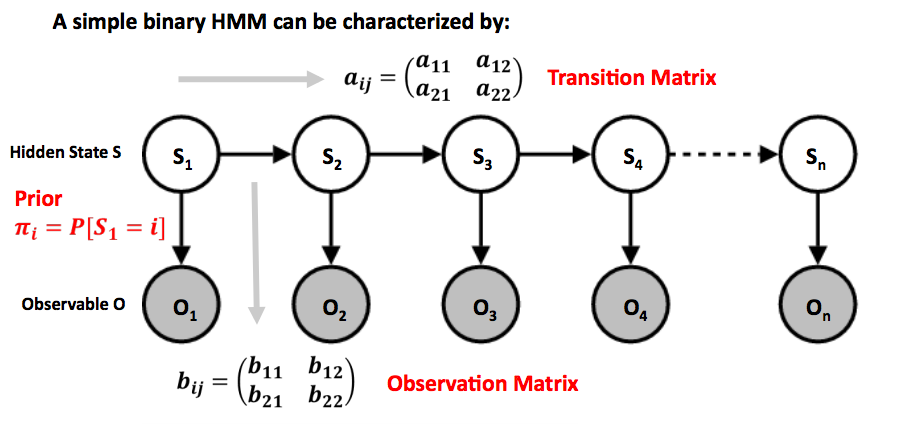
\includegraphics[scale=0.35]{p1.png}
\caption{Hidden Markov Model}
\end{figure}
}

\frame{\frametitle{Traditional Bayesian Knowledge Tracing}
\begin{figure}
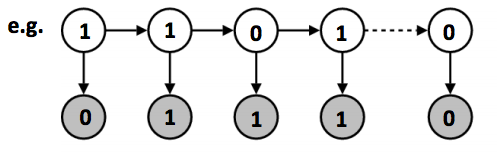
\includegraphics[scale=0.35]{p2.png}
\caption{Bayesian Knowledge Tracing}
\end{figure}
}


\frame{\frametitle{Parameters of the BKT}
The BKTs are caracterized with the Prior distribution, the Transition Matrix and The Emission (Observation) matrix. In this project, are equivalent to:
\begin{itemize}
\item \textbf{P-init}: Initial a priori of knowing the skill $p(L_0)$
\item \textbf{P-transit}: Probability of each student to transition from \textit{not known} to \textit{known} $p(T)$
\item \textbf{P-slip}: Probability to make a mistake when applying a known skill $p(S)$
\item \textbf{P-guess}: Probability of correctly applying a not-known skill $p(G)$ 
\end{itemize} 
}

\frame{\frametitle{Equivalence with HMM}
The P-slip and P-guess are components of the Emission matrix and P-transit of the Transition matrix.
\begin{figure}
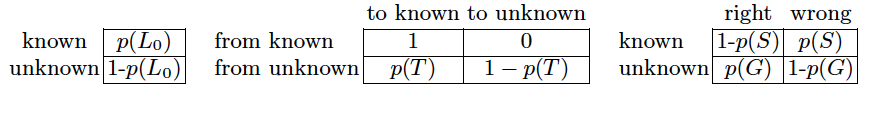
\includegraphics[scale=0.35]{p3.png}
\caption{Transition and Emission matrix of BKT}
\end{figure}
}


\frame{\frametitle{Individualized Bayesian Knowledge Tracing}
Idea:
\begin{itemize}
\item All data for the students practicing skill $k$ would be used to fit four BKT parameters for that skill: $P^k$
\item All data for student $u$ will be used to fit four parameters for that student $P_u$
\item Build a function to yield a value $p^k_u$ 
\end{itemize}  
}


\frame{\frametitle{Problems and fitting}
How to update the parameters?

\textbf{First attemps:} Expectation maximization method (EM), Conjugate gradient methods, but
EM doesn’t optimize a likelihood of the observations given BKT parameters. 

\textbf{Other approaches:}

Bayesian approaches (HMC, MCMC)


}

\end{document}